\documentclass[journal]{vgtc}                % final (journal style)
%\documentclass[review,journal]{vgtc}         % review (journal style)
%\documentclass[widereview]{vgtc}             % wide-spaced review
%\documentclass[preprint,journal]{vgtc}       % preprint (journal style)
%\documentclass[electronic,journal]{vgtc}     % electronic version, journal

%% Uncomment one of the lines above depending on where your paper is
%% in the conference process. ``review'' and ``widereview'' are for review
%% submission, ``preprint'' is for pre-publication, and the final version
%% doesn't use a specific qualifier. Further, ``electronic'' includes
%% hyperreferences for more convenient online viewing.

%% Please use one of the ``review'' options in combination with the
%% assigned online id (see below) ONLY if your paper uses a double blind
%% review process. Some conferences, like IEEE Vis and InfoVis, have NOT
%% in the past.

%% Please note that the use of figures other than the optional teaser is not permitted on the first page
%% of the journal version.  Figures should begin on the second page and be
%% in CMYK or Grey scale format, otherwise, color shifting may occur
%% during the printing process.  Papers submitted with figures other than the optional teaser on the
%% first page will be refused.

%% These three lines bring in essential packages: ``mathptmx'' for Type 1
%% typefaces, ``graphicx'' for inclusion of EPS figures. and ``times''
%% for proper handling of the times font family.

\usepackage{mathptmx}
\usepackage{graphicx}
\usepackage{times}
\usepackage{balance}
\usepackage[nooneline,hang,it,IT]{subfigure}

%% We encourage the use of mathptmx for consistent usage of times font
%% throughout the proceedings. However, if you encounter conflicts
%% with other math-related packages, you may want to disable it.

%% This turns references into clickable hyperlinks.
\usepackage[bookmarks,backref=true,linkcolor=black]{hyperref} %,colorlinks
\hypersetup{
  pdfauthor = {},
  pdftitle = {},
  pdfsubject = {},
  pdfkeywords = {},
  colorlinks=true,
  linkcolor= black,
  citecolor= black,
  pageanchor=true,
  urlcolor = black,
  plainpages = false,
  linktocpage
}

%% If you are submitting a paper to a conference for review with a double
%% blind reviewing process, please replace the value ``0'' below with your
%% OnlineID. Otherwise, you may safely leave it at ``0''.
\onlineid{0}

%% declare the category of your paper, only shown in review mode
\vgtccategory{Research}

%% allow for this line if you want the electronic option to work properly
\vgtcinsertpkg

%% In preprint mode you may define your own headline.
%\preprinttext{To appear in an IEEE VGTC sponsored conference.}

%% Paper title.

\title{AiPoker - Implementation of a Poker Agent}

%% This is how authors are specified in the journal style

%% indicate IEEE Member or Student Member in form indicated below
\author{John Holl\'en, Robin Berntsson, Simon Bergst\"om}
\authorfooter{
%% insert punctuation at end of each item
\item
 John Holl\'en, Robin Berntsson, Simon Bergstr\"om
}

%% Abstract section.
\abstract{ 
We will probably write this section the last thing we do. 
}
%% Keywords that describe your work. Will show as 'Index Terms' in journal
%% please capitalize first letter and insert punctuation after last keyword
\keywords{Monte Carlo Tree Search, Texas Hold'em}



%%%%%%%%%%%%%%%%%%%%%%%%%%%%%%%%%%%%%%%%%%%%%%%%%%%%%%%%%%%%%%%%
%%%%%%%%%%%%%%%%%%%%%% START OF THE PAPER %%%%%%%%%%%%%%%%%%%%%%
%%%%%%%%%%%%%%%%%%%%%%%%%%%%%%%%%%%%%%%%%%%%%%%%%%%%%%%%%%%%%%%%%

\begin{document}

%% The ``\maketitle'' command must be the first command after the
%% ``\begin{document}'' command. It prepares and prints the title block.

%% the only exception to this rule is the \firstsection command
\firstsection{Background}
\maketitle 
Texas Hold'em is a popular variant of poker, not just to play with friends but also online against other people for money. Poker belongs with the most difficult kind of card game to solve discretely since it is an stochastic game with imperfect information. The challenge of creating the best poker agent has attracted a lot of people and is a popular subject in AI development.

There are many different games today and the strategy to solve these games depends on the type of game. In game theory games can be classified due to the knowledge if the transition to a new state within the game depends on a stochastic process and if there is some hidden information. Poker belongs with the most difficult kind of card game to solve discretely since it is an stochastic game with imperfect information.
\\*\\*
\textbf{Perfect Information vs Imperfect Information}\\*
In perfect information games both players can observe the complete state of the game at any given time, this is the case in games such as Chess and Go. Contrary to this we have imperfect information games where each player is unable to observe the complete state, one example for this is poker were neither player can see the other players pocket cards.
\\*\\*
\textbf{Deterministic vs Stochastic}\\*
In deterministic games the next state of the game is uniquely determined by an action taken at the current state. In contrast, a stochastic game is a game where the player don't have control over the transition to the next state. For example in poker where the new cards is drawn from a scrambled deck. 

\begin{table}[h]
\begin{tabular}{lll}
              & Perfect Information  & Imperfect Information \\
Deterministic & Chess, Go            & Battleships           \\
Stochastic    & Backgammon, Monopoly &                      
\end{tabular}
\caption{\label{tab:table1} Table showing different categories of games.}
\end{table}

In general imperfect information games require more complex reasoning than perfect information games and deterministic games is easier than stochastic. This places Chess and go in the ?easier? category while poker is in the ?hardest? one.

The theory behind Monte Carlo search trees will be studied within this project and tested as a part of the logic that will determine the actions of the poker agent. Smaller algorithms to improve the logic for the AI will be tested and implemented in combination of the Monte Carlo Search Tree to create the best possible poker agent.

\subsection{Monte Carlo Methods}
Monte Carlo methods is a class of algorithms that rely on random sampling to obtain a numerical estimate of a complicated problem. The method was invented by Stanislaw Ulam while working with the nuclear weapon program at Los Alamos in the 1940s [REF!]. 
\begin{figure}[here]
  \begin{center}
    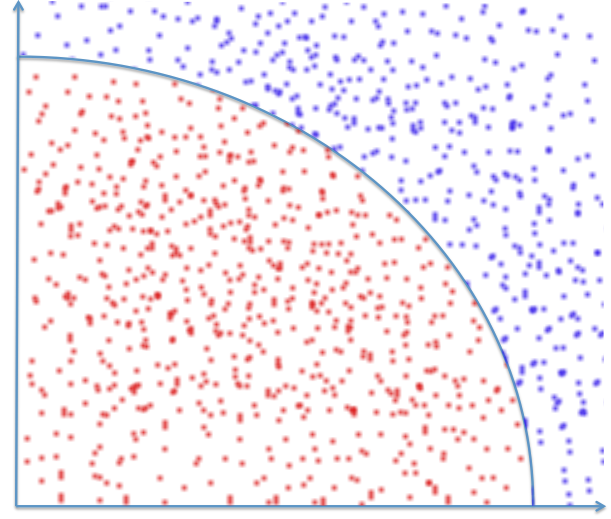
\includegraphics[scale=0.35]{img/integralexample.png}
    \caption{\label{fig:integralex} An illustration of how to determine the value of an integral with the help of Monte Carlo methods.}
  \end{center}
\end{figure}
 
One possible use for Monte Carlo methods is to determine the value of an integral as illustrated in fig(\ref{fig:integralex}). By randomly placing dots and label them as under or over the function value we can get an estimate of the area by taking the area of the square encapsulating the function times the ratio between the number of points under the function with those above the function. The approximated value given by the Monte Carlo simulation will converge to the correct value as the number of sample points goes to infinity.

The insight that random sampling can be used to solve problems that is too complex to solve analytically can be used to evaluate the best action in huge game trees. For a given node N we can estimate its value by running a number of simulations of how the game may end from that node. The result from those simulations can then be used to give an approximation for the value of that state and as N grows it will converge to the result from a Minimax search. 

Monte-Carlo methods for game trees have made huge improvements for game which was previously very hard for AIs. One example is Go in which bots powered with MCTS now can reach the highest level of play.

\section{Theory}
\subsection{Texas Hold'em no Limit}
There are many forms of poker, with the most popular being the Texas Hold?em. Texas Hold?em can be played in two different styles, limited and no-limits. In limited poker the amount you bet or raise is fixed, and there is an upper amount of times that you can raise. However in no limited there is no restriction to the amount of money or times you can raise.

\subsubsection{Main Concept}
The game aims to win as many hands as possible and to get the opponent(s) coins and when a player is out of coins he has lost the game. When everyone except one player has run out of coins the game is over and a winner is designated.

Each player gets two cards and the player with the best five combination of the cards on the players hand and the cards on the poker board wins the round. 

In order to always have money in the pot of each round and take away the risk of a player to be to defensive and never bet a small fee i circulating around the players through the game called the blind. The blind is two amounts called big and small blind. When the game starts a player gets randomly selected to pay the big blind and the player next on the left to him gets to pay the small blind. When a round  is played the blind moves one step to the left so the person who had the small blind get to pay the big blind this turn and the player left to him gets the small blind. If there is only two players they just switch big and small blind every round. The big blind is the double amount of the small blind and is a pre set sum.

The game consist of five stages where the players can decide how to proceed in the game.
These stages are pre-flop, flop, turn, river and showdown.

\subsubsection{The Game Stages}

\textbf{Pre Flop}\\*
In this stage the players gets their two cards from the dealer called the pocket cards and the player who is first are able to either bet, call if he has not paid the big blind, check if he has paid the big blind or fold. Since you can not form a five combination of cards yet only a speculation of how good your pocket cards is. If a player bets or raise all other players get the opportunity to either call,raise or fold max three times, after that the player who has not fold moves on to the flop.
\\*\\*
\textbf{Flop}\\*
The flop is when the dealer puts out the three first cards on the table who is visible for all players and makes it possible for all players to form their first five combination and calculate how good cards they have. Like in the pre flop phase all players will make moves in the same procedure to see which who are still left to the turn phase.
\\*\\*
\textbf{Turn}\\*
Now the dealer adds one card to the flop so its totally four visible card on the table. The players could then form a new five card combination to see how good their cards are. Same as previous steps there will be some betting before going on to the river.
\\*\\*
\textbf{River}\\*
The dealer add another card so there is five cards on the table for the player to make their best five combinations of cards with. This was the last card that will be distributed so after some more betting there is time for the showdown.
\\*\\*
\textbf{Showdown}\\*
In this phase the final betting is completed and the players who has not folded will now show their cards in order to decide who is the winner of this round. The winner will get the full pot and then a new round will start with the pre flop.
\\*\\*
\textbf{The different five combination of cards}\\*
There are nine different types of combination of cards and here they are listed in descending order[3]:
\begin{itemize}
  \item \textit{Straight Flush}: When you have a five cards in a consecutive order of value with the same suit. If more than one player have the Straight Flush the player with the highest values of their cards wins, and the best type is the Royal Straight Flush when you have Ace,King,Queen and Knight with the same suit.
  \item \textit{Four of a kind}: It is a hand that contains four of the same number, which means in all the different suits. If different players have the same type of hand the hand with the highest four of a kind wins.
  \item \textit{Full House}:   It is a hand where you have three cards of the same value in combination with two other cards that have the similar value. If more than one player have a Full House the player with the highest value three of a kind wins, if two players have the same three of a kind the player with the highest value of one pair wins.
  \item \textit{Flush}: It is when you have five cards with the same suit, if more than one player have a flush the one which have the highest card wins. If they have the same highest card then the the second highest card is checked and so on.
  \item \textit{Straight}: When you have a five cards in a consecutive order of value and if more than one player have a Straight then the player with the highest card wins.
  \item \textit{Three of a Kind}: When you have three cards of the same value, if more than one player has a Three of a kind then the player with the highest value of the cards wins.
  \item \textit{Two Pair}: When you have two card with the same values in combination with two other cards with the same values. In other words they have two pair of cards, if more than one player have a two pair the player with the highest pair has the best hand between them.
  \item \textit{One Pair}: When you have one pair of cards, if more than one player have a one pair the player with the highest pair has the best hand between them.
  \item \textit{High Card}: If the card does not match any of the types above then the card with the highest value is considered.

\end{itemize}

\subsection{Characteristics of a Poker Player}
Like previously described poker is a stochastic game, that makes it very hard to control and to define what a good poker player is. A good poker player does not always need to be the one who is playing optimally. A good poker player is hard to define but some of the main characteristics of a good player is that he is enjoying the game, can read his opponents strategy or way of playing and also know when having a good hand to play with.[REF!]

A player who tries to maximise his winnings will have to use bluffing. The reason for this is two-fold. First, since betting is often associated with holding strong cards, opponents might be tricked to give up a stronger hand. By betting on his weaker cards the bluffing player might win a pot that he would otherwise lose because he holds the weakest cards. Second and most interestingly: if a player is known to only bet with strong cards, his opponents can just fold whenever he bets and he will have a hard time winning money with his strong cards.  

\section{Method}
\subsection{Basic Game Engine}
In order to even begin implementing an AI, the core poker game had to be implemented first. For simplicity the game implemented in this study is a two player game where a human player faces a computer AI. The player who starts is chosen at random when the game is started. The player that starts then puts one dollar in to the pot. The other player puts two dollars in the pot. Then the game is turn based like ordinary Texas Hold?em, the players can bet, check, call, raise and fold. And after each betting round cards are dealt to the table and the players combine the cards on hand with the cards on the table in order to get the strongest hand possible. 

An very easy poker agent was implemented that played totally random was created in the purpose of testing the implemented game and later on the AI poker agent that was going to be implemented with Monte Carlo and other interesting poker algorithms(See 3.2.).

\subsection{AI-techniques}
A couple of different AI-techniques were implemented in this study. They are described in this section. Also some tests were the different AIs were competing against each other were made.
\subsubsection{Monte Carlo Tree Search}
MCTS is a best-first search strategy. Every node in the tree contain two values, an estimate of the expected value $V(P)$ of the reward $r(P)$ and the number of times the node have been visited $n_{i}$. MCTS only starts with the root node and incrementally build the tree by repeating the following 4 steps.\\*\\*
\textbf{Selection}
\\*Selection is made by starting from the root node and then recursively select nodes until a leaf node is reached (this does not have to be a leaf of the game tree). To determine which node is the optimal one, the upper confidence bounds (UCB1) formula is used: 

\begin{equation} \label{eq:upperconfidence}
	v_{i} + C \cdot \sqrt{\frac{\ln N}{n_{i}}}
\end{equation}
The first term vi is the estimated value of the node and is responsible for exploitation of good nodes, the second term is made up by the total number of visits of the parent node $N$ and the total number of visits of the current node $n_{i}$. The constant $C$ allows tuning of the exploration-exploitation trade-off. 
\\*\\*
\textbf{Expansion}
\\*If the leaf node reached is not an terminating node, which means that the game is not over at the current node. Then create one or more child nodes from the node currently at. This step is illustrated in fig(\ref{fig:expansion}).
\begin{figure}[here]
  \begin{center}
    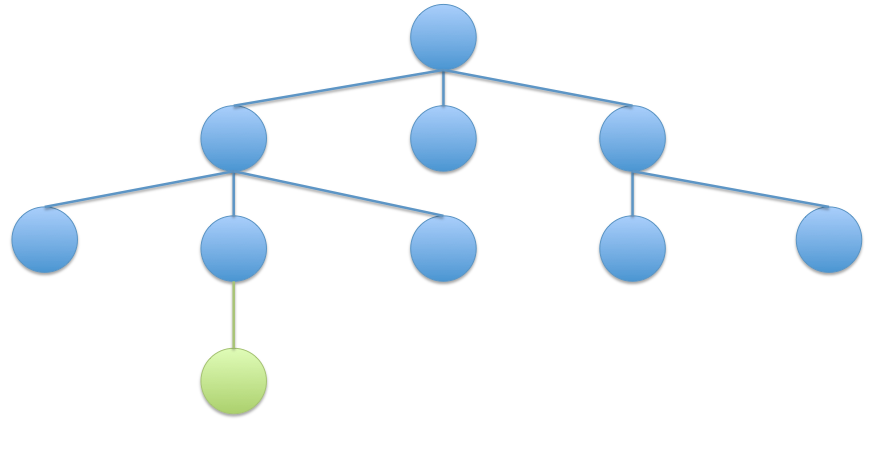
\includegraphics[scale=0.28]{img/tree1.png}
    \caption{\label{fig:expansion} Illustration of how the green node is added to the tree.}
  \end{center}
\end{figure}
\\*
\textbf{Simulation}
\\*The third step in MCTS is the simulation step. Here a game is simulated from the state in the new node until a result is achieved. The value of the reached result is recorded.
\\*\\*
\textbf{Backpropagation}
\\*The last step is to update the expected value and the selection counter for all nodes along the explored path by backpropagating the recorded result from the simulation step. This step is illustrated in fig(\ref{fig:backprop}).
\begin{figure}[here]
  \begin{center}
    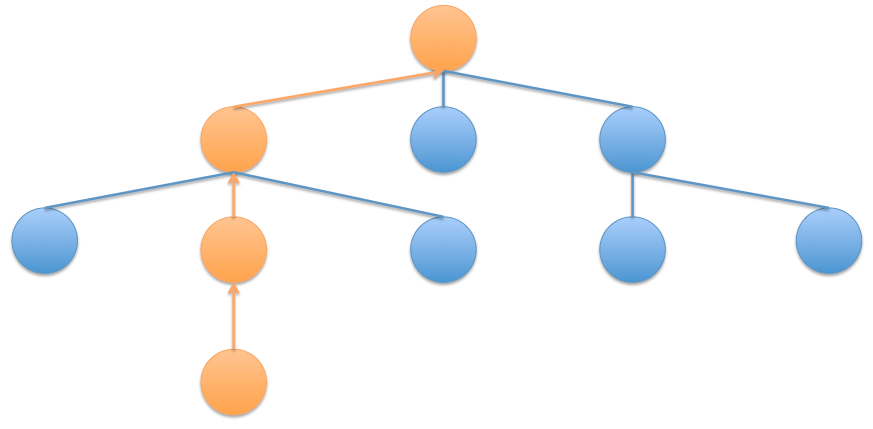
\includegraphics[scale=0.28]{img/tree2.png}
    \caption{\label{fig:backprop} Illustration of how the path to the node is updated with the score from the simulation in the whole tree.}
  \end{center}
\end{figure}
When the back propagation step is finished the whole chain starts over again starting with the selection step. This is done until the either the game tree is fully searched or a time limit is reached. The fact that MCTS can give a result after a given time is a result of it being anytime, that is it will give a valid solution to the problem even if it is interrupted before it is finished. However the quality of the solution is an estimate and is expected to be better the more time the MCTS keeps running.

One problem that is introduced with the MCTS is how to run the simulation step. Here we have to select the moves for each player until the end of the game. One solution could be to just select random moves, this can work well for simple games but for games as complex as poker this will lead to bad results. This implies that we somehow have to model the opponent to be able to determine the correct actions in the simulation.  

\subsubsection{Hand Strength}
Since Monte Carlo is a heuristic search which simulate a set of outcomes in a game to calculate what action to make the logic so far does not consider how good  the cards on the agents hand is compared to other hands. To add this logic to the agent an algorithm could be used that would return a probability of how strong the current hand cards is with the cards on the table. This probability of the Hand Strength may, at the earliest be calculated the the flop has been shown. [REF!]

The Hand Strength is calculated by comparing the cards on the hand with all possible combination of two cards that the opponent can have and sum the time the agents cards wins compared to the opponent and divide by the number of combinations that was simulated.

\subsubsection{Hand Potential}
The hand potential algorithm calculates the quality of the hand as the game goes on. The algorithm is similar to the hand strength algorithm. The difference is that the hand potential algorithm considers all possible cards that have not been revealed yet. It is also heavier to calculate since it has to go through every possible combination of cards that could possibly end up on the table. It also takes into account every possible card the opponent might have on hand.

\subsubsection{Effective Hand Strength}
By combining the hand strength with the hand potential a probability of winning can be calculated, and this is called the effective hand strength and is calculated as following:

\begin{equation} \label{EHS}
	EHS = HS \cdot (1-NPot) \cdot PPOT
\end{equation}

\subsection{Implementation}
\subsubsection{Main Design}
The application implemented in this study was implemented in Javascript using the library Three.js for visualization. Three.js is a webGL library which provides high level functions for creating a 3D scene.

The application is implemented in an object oriented manner. The main application file is called main.js and it is here the scene is created and where all the other classes needed are initialized. The file main.js also contains all the click listeners for the buttons the human player uses to do moves. An overview over the game architecture is shown in fig(\ref{fig:arcitect}). 
\begin{figure}[here]
  \begin{center}
    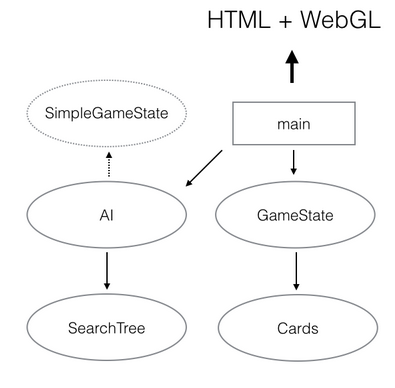
\includegraphics[scale=0.50]{img/arcitect.png}
    \caption{\label{fig:arcitect} Illustration of how the path to the node is updated with the score from the simulation in the whole tree.}
  \end{center}
\end{figure}

\subsubsection{Game}
The main.js file is first painting the poker table and all buttons on the page, when you click the start button a GameState object and a AI will be created.
The poker game is originated from the GameState object which only consists of a Cards object and functions for every state of the poker game Texas Hold'em. The game is created for two players where one player is an AI agent and the other player is the client controlled by a human. The Cards object consist of a full deck of cards and all methods needed for playing Texas Hold'em like shuffle the deck of cards, deliver the flop, turn card, river card and cards for the players.

\section{Result}
\subsection{The Game}
The result of this study is a Texas Hold'em game with an AI implemented using several different AI techniques and combining them together. The AI in the interactive game is using Monte Carlo Tree Search together with Hand Strength as a heuristic. The game is fully playable with an opponent that is somewhat realistic in the way it chooses what move to make. The 3D-scene is used to visualise the poker table, and it also shows the cards on hand. This is shown in fig(\ref{fig:3dscene}).
\begin{figure}[here]
  \begin{center}
    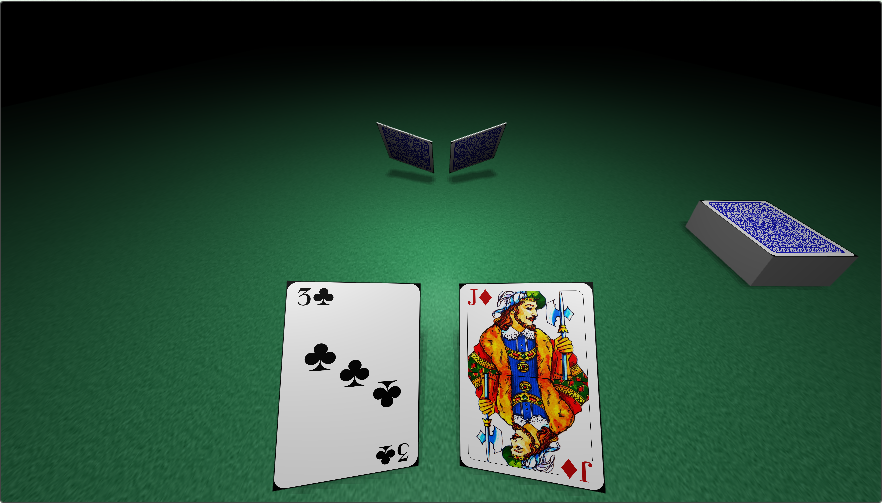
\includegraphics[scale=0.27]{img/3dscene.png}
    \caption{\label{fig:3dscene} The 3D-scene in the final version showing the player's cards on hand.}
  \end{center}
\end{figure}

To the left of the 3D-scene there are some additional UI-elements. these are the buttons telling the player what moves he or she can make. By pressing one of these buttons the player will make a move. The coloured buttons indicate that a move is valid. The greyed out buttons indicate invalid moves. The buttons are shown in fig(\ref{fig:ui1}).
\begin{figure}[here]
  \begin{center}
    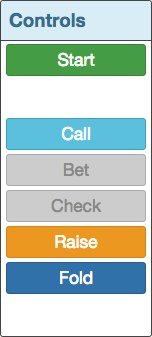
\includegraphics[scale=0.50]{img/ui1.png}
    \caption{\label{fig:ui1} The player controls, placed to the left of the 3D-scene. Greyed out buttons indicate an invalid move.}
  \end{center}
\end{figure}

To the right of the 3D-scene some information is shown. Information about money is shown in the upper box. How much money each player has, and how much money there is currently on the table. This information box is illustrated in fig(\ref{fig:ui2}).
\begin{figure}[here]
  \begin{center}
    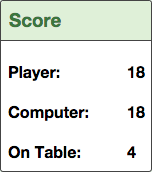
\includegraphics[scale=0.50]{img/ui2.png}
    \caption{\label{fig:ui2} The score board giving the player information about the money currently in play.}
  \end{center}
\end{figure}

Right below the score board, the enemy log is placed. It keeps track of what the computer does each time it makes a move. Since this is quite hard to visualise the decision was made to print the computer's move in text every time it makes a move. The enemy log is shown in fig(\ref{fig:ui3}).
\begin{figure}[here]
  \begin{center}
    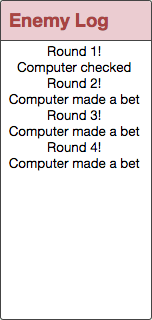
\includegraphics[scale=0.50]{img/ui4.png}
    \caption{\label{fig:ui3} The enemy log, showing what the computer has done each round.}
  \end{center}
\end{figure}

\subsection{AI}
Since a number of algorithms were implemented in this study several results were achieved and therefore comparisons between the different approaches can be made. During this study, the different AI were put against each other playing several games. The following setups were made: 
\begin{itemize}
\item \textit{Monte Carlo + Hand Strength} vs \textit{Random Agent}
\item \textit{Effective Hand Strength} vs \textit{Monte Carlo + Hand Strength}
\item \textit{Monte Carlo} vs \textit{Monte Carlo + Hand Strength}
\item \textit{Monte Carlo + Hand Strength} vs \textit{Human Player}
\end{itemize}

\section{Conclusion}



\begin{thebibliography}{9}

\bibitem{byron}
  Byron L., Wattenberg M.
  \emph{Stacked graphs - Geometry \& Aesthetics}.
  IEEE Transactions on Visualization and Computer Graphics archive
Volume 14 Issue 6,
Pages 1245-1252. IEEE Educational Activities Department Piscataway, NJ, USA
ISSN: 1077-2626.
  2008.

\bibitem{reynolds}
  Reynolds A. P., Richards G., Rayward-Smith V. J.
  \emph{The Application of K-medoids and PAM to the Clustering of Rules}.
  In: Intelligent Data Engineering and Automated Learning - IDEAL 2004. Lecture Notes in Computer Science, 3177 . Springer-Verlag, pp. 173-178. ISBN 978-3-540-22881-3,
  2004.

\end{thebibliography}

\end{document}
